\documentclass[11pt]{scrartcl}

\usepackage[utf8]{inputenc}

\usepackage[T1]{fontenc}
\usepackage[french]{babel}

\usepackage{textcomp}
\usepackage{amsmath}
\usepackage{amssymb}
\usepackage{mathtools}
\usepackage{siunitx}
\usepackage{lmodern}
\usepackage{graphicx}
\usepackage{tabularx}

\usepackage{microtype}
\usepackage[parfill]{parskip}
\usepackage[hidelinks]{hyperref}

\title{Vie artificielle}
\subtitle{Automates cellulaires}

\author{Lieselotte \textsc{Marchal}}

\begin{document}
    \maketitle
    
    \section{Blob}
        \subsection{Modélisation du monde}
            Le monde est constitué de texels à trois composantes :
            \begin{itemize}
                \item Un booléen indiquant si la case est occupée par un agent ;
                \item Un réel indiquant l'orientation d'un tel agent ;
                \item Un réel indiquant le taux de matériel présent sur la case.
            \end{itemize}
        
        \subsection{Règles de simulation}
            À chaque pas de temps, les agents sont d'abord déplacés de \texttt{STEP\_LENGTH}.
            Plusieurs agents allants sur la même case sont combinés en un seul agent ; le type de combinaison est déterminée par l'option \texttt{BOUNCE}.
            
            Le matériel est ensuite diffusé uniformément sur un côté de \texttt{DIFFUSION\_SIZE}, puis évaporé selon \texttt{RETENTION\_RATE}.
            
            Les agents déposent enfin \texttt{DEPOSIT\_AMOUNT} matériel sur chaque case dans un carré de côté \texttt{DEPOSIT\_SIZE}, puis se réorientent
            selon les paramètres \texttt{SENSOR\_DISTANCE}, \texttt{SENSOR\_SIZE} et \texttt{SENSOR\_ANGLE}.
        
        \subsection{Propriétés}
            Du fait que certains agents se combinent en un seul, l'automate n'est pas réversible.
            Comme des agents ne sont jamais recréés, la densité de l'automate est décroissante et tend vers une constante positive.
        
        \subsection{Simulation}
            Les figures~\ref{fig:phy-rgb} et \ref{fig:phy-hsv} montrent une simulation à $t = 5000$ qui converge en un vaisseau spatial allant
            indéfiniment à droite.
            
            \begin{figure}[h]
                \centering
                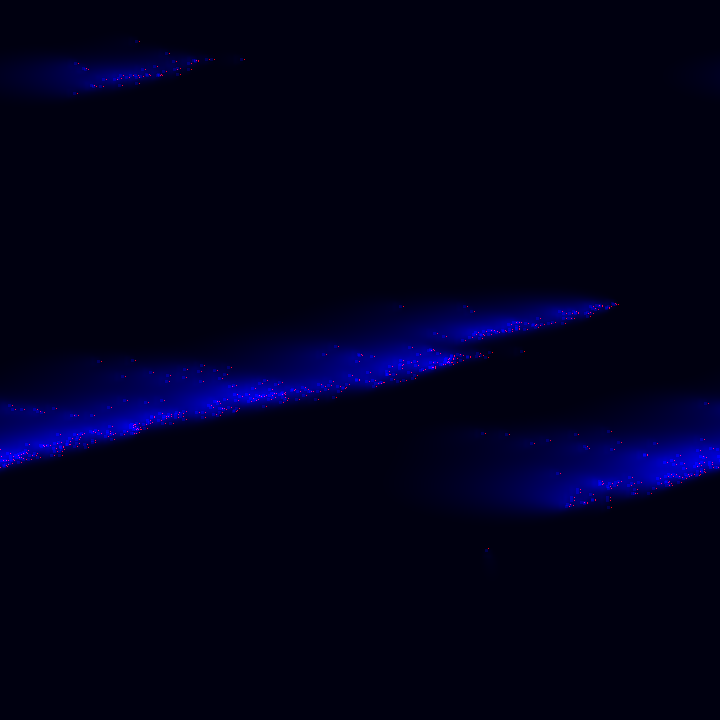
\includegraphics[width=\textwidth]{physarum_rgb}
                \caption{Blob ; en bleu la concentration de matériel, en rouge les agents.}\label{fig:phy-rgb}
            \end{figure}
            
            \begin{figure}[h]
                \centering
                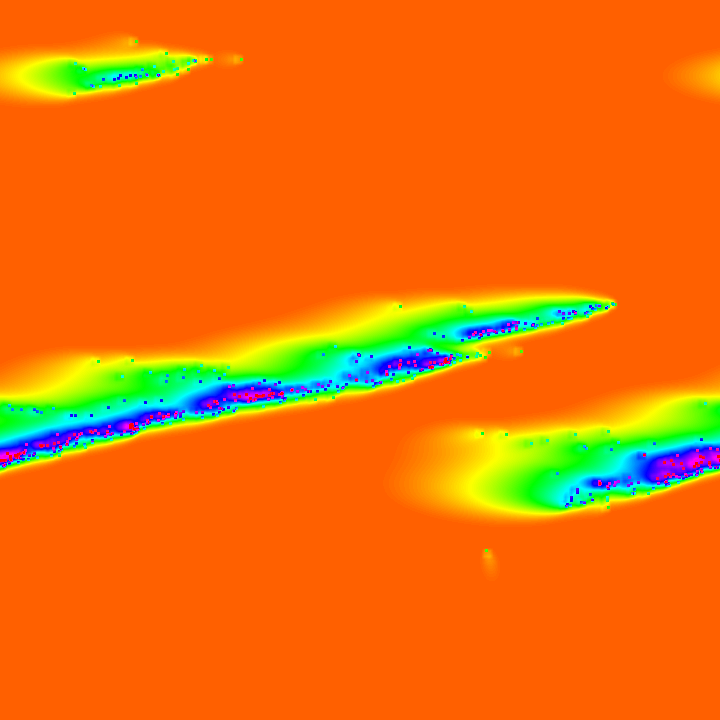
\includegraphics[width=\textwidth]{physarum_hsv}
                \caption{Blob ; concentration de matériel. Les agents viennent d'émettre et sont ainsi visibles.}\label{fig:phy-hsv}
            \end{figure}
    
    \section{Tesselation}
        \subsection{Modélisation du monde}
            Le monde est constitué de texels à trois composantes :
            \begin{itemize}
                \item Une énumération pour le type d'agent (A, B, C, D, ou X (pas d'agent)).
                \item Un réel indiquant l'orientation d'un tel agent ;
                \item Un réel indiquant le taux de catalyseur (émit par C) présent sur cette case,
                      ou la durée de vie restante de l'agent si c'est une membrane (C).
            \end{itemize}
            
            La cellule est centrée au centre du monde, et est de rayon \texttt{CELL\_RADIUS}.
            La membrane est générée avec une durée de vie restante aléatoire.
        
        \subsection{Règles de simulation}
            À chaque pas de temps, les membranes perdent \texttt{MEMBRANE\_DEGRADATION\_SPEED} points de vie et se transforment en D si ce nombre
            est descendu à zéro.
            
            Le taux de catalyseur est recalculé selon \texttt{CATALYST\_RANGE}.
            
            Les agents A sont transformés en B s'ils sont sur une case suffisamment catalysée.
            
            Les agents A, B et D sont déplacés de \texttt{COMPOUND\_SPEED} sur des cases sans agent.
            En cas de collision, B remplace A qui remplace D, de telle sorte à ce que l'agent le plus important reste en vie.
            
            Si un agent B est suffisament proche d'un ou de plusieurs trous, alors il les rebouche tous en devenant C.
        
        \subsection{Propriétés}
            Cet automate n'est pas non plus réversible, puisque plusieurs agents se combinent toujours en un seul.
        
        \subsection{Simulation}
            La catalyse est représentée en bleu, l'agent A en rouge, et l'agent B en vert.
            Les agents C et D ne sont pas représentés.
    
\end{document}

